
%% mypaper.tex
%% V1.4b
%% 2015/08/26
%% by Michael Shell
%% see http://www.michaelshell.org/
%% for current contact information.
%%
%% This is a skeleton file demonstrating the use of IEEEtran.cls
%% (requires IEEEtran.cls version 1.8b or later) with an IEEE 
%% Transactions on Magnetics journal paper.
%%
%% Support sites:
%% http://www.michaelshell.org/tex/ieeetran/
%% http://www.ctan.org/pkg/ieeetran
%% and
%% http://www.ieee.org/

%%*************************************************************************
%% Legal Notice:
%% This code is offered as-is without any warranty either expressed or
%% implied; without even the implied warranty of MERCHANTABILITY or
%% FITNESS FOR A PARTICULAR PURPOSE! 
%% User assumes all risk.
%% In no event shall the IEEE or any contributor to this code be liable for
%% any damages or losses, including, but not limited to, incidental,
%% consequential, or any other damages, resulting from the use or misuse
%% of any information contained here.
%%
%% All comments are the opinions of their respective authors and are not
%% necessarily endorsed by the IEEE.
%%
%% This work is distributed under the LaTeX Project Public License (LPPL)
%% ( http://www.latex-project.org/ ) version 1.3, and may be freely used,
%% distributed and modified. A copy of the LPPL, version 1.3, is included
%% in the base LaTeX documentation of all distributions of LaTeX released
%% 2003/12/01 or later.
%% Retain all contribution notices and credits.
%% ** Modified files should be clearly indicated as such, including  **
%% ** renaming them and changing author support contact information. **
%%*************************************************************************


% *** Authors should verify (and, if needed, correct) their LaTeX system  ***
% *** with the testflow diagnostic prior to trusting their LaTeX platform ***
% *** with production work. The IEEE's font choices and paper sizes can   ***
% *** trigger bugs that do not appear when using other class files.       ***                          ***
% The testflow support page is at:
% http://www.michaelshell.org/tex/testflow/



\documentclass[journal,transmag]{IEEEtran}
%
% If IEEEtran.cls has not been installed into the LaTeX system files,
% manually specify the path to it like:
% \documentclass[journal]{../sty/IEEEtran}





% Some very useful LaTeX packages include:
% (uncomment the ones you want to load)


% *** MISC UTILITY PACKAGES ***
%
%\usepackage{ifpdf}
% Heiko Oberdiek's ifpdf.sty is very useful if you need conditional
% compilation based on whether the output is pdf or dvi.
% usage:
% \ifpdf
%   % pdf code
% \else
%   % dvi code
% \fi
% The latest version of ifpdf.sty can be obtained from:
% http://www.ctan.org/pkg/ifpdf
% Also, note that IEEEtran.cls V1.7 and later provides a builtin
% \ifCLASSINFOpdf conditional that works the same way.
% When switching from latex to pdflatex and vice-versa, the compiler may
% have to be run twice to clear warning/error messages.






% *** CITATION PACKAGES ***
%
%\usepackage{cite}
% cite.sty was written by Donald Arseneau
% V1.6 and later of IEEEtran pre-defines the format of the cite.sty package
% \cite{} output to follow that of the IEEE. Loading the cite package will
% result in citation numbers being automatically sorted and properly
% "compressed/ranged". e.g., [1], [9], [2], [7], [5], [6] without using
% cite.sty will become [1], [2], [5]--[7], [9] using cite.sty. cite.sty's
% \cite will automatically add leading space, if needed. Use cite.sty's
% noadjust option (cite.sty V3.8 and later) if you want to turn this off
% such as if a citation ever needs to be enclosed in parenthesis.
% cite.sty is already installed on most LaTeX systems. Be sure and use
% version 5.0 (2009-03-20) and later if using hyperref.sty.
% The latest version can be obtained at:
% http://www.ctan.org/pkg/cite
% The documentation is contained in the cite.sty file itself.






% *** GRAPHICS RELATED PACKAGES ***
%
\ifCLASSINFOpdf
   \usepackage[pdftex]{graphicx}
   \graphicspath{{../pdf/}{../jpeg/}}
   \DeclareGraphicsExtensions{.pdf,.jpeg,.png,.jpg}
   \usepackage[utf8]{inputenc}
%   \usepackage{assymb, amsmath, amsthm}

\else
  % or other class option (dvipsone, dvipdf, if not using dvips). graphicx
  % will default to the driver specified in the system graphics.cfg if no
  % driver is specified.
  % \usepackage[dvips]{graphicx}
  % declare the path(s) where your graphic files are
  % \graphicspath{{../eps/}}
  % and their extensions so you won't have to specify these with
  % every instance of \includegraphics
  % \DeclareGraphicsExtensions{.eps}
\fi
% graphicx was written by David Carlisle and Sebastian Rahtz. It is
% required if you want graphics, photos, etc. graphicx.sty is already
% installed on most LaTeX systems. The latest version and documentation
% can be obtained at: 
% http://www.ctan.org/pkg/graphicx
% Another good source of documentation is "Using Imported Graphics in
% LaTeX2e" by Keith Reckdahl which can be found at:
% http://www.ctan.org/pkg/epslatex
%
% latex, and pdflatex in dvi mode, support graphics in encapsulated
% postscript (.eps) format. pdflatex in pdf mode supports graphics
% in .pdf, .jpeg, .png and .mps (metapost) formats. Users should ensure
% that all non-photo figures use a vector format (.eps, .pdf, .mps) and
% not a bitmapped formats (.jpeg, .png). The IEEE frowns on bitmapped formats
% which can result in "jaggedy"/blurry rendering of lines and letters as
% well as large increases in file sizes.
%
% You can find documentation about the pdfTeX application at:
% http://www.tug.org/applications/pdftex




% *** MATH PACKAGES ***
%
%\usepackage{amsmath}
% A popular package from the American Mathematical Society that provides
% many useful and powerful commands for dealing with mathematics.
%
% Note that the amsmath package sets \interdisplaylinepenalty to 10000
% thus preventing page breaks from occurring within multiline equations. Use:
%\interdisplaylinepenalty=2500
% after loading amsmath to restore such page breaks as IEEEtran.cls normally
% does. amsmath.sty is already installed on most LaTeX systems. The latest
% version and documentation can be obtained at:
% http://www.ctan.org/pkg/amsmath





% *** SPECIALIZED LIST PACKAGES ***
%
%\usepackage{algorithmic}
% algorithmic.sty was written by Peter Williams and Rogerio Brito.
% This package provides an algorithmic environment fo describing algorithms.
% You can use the algorithmic environment in-text or within a figure
% environment to provide for a floating algorithm. Do NOT use the algorithm
% floating environment provided by algorithm.sty (by the same authors) or
% algorithm2e.sty (by Christophe Fiorio) as the IEEE does not use dedicated
% algorithm float types and packages that provide these will not provide
% correct IEEE style captions. The latest version and documentation of
% algorithmic.sty can be obtained at:
% http://www.ctan.org/pkg/algorithms
% Also of interest may be the (relatively newer and more customizable)
% algorithmicx.sty package by Szasz Janos:
% http://www.ctan.org/pkg/algorithmicx




% *** ALIGNMENT PACKAGES ***
%
%\usepackage{array}
% Frank Mittelbach's and David Carlisle's array.sty patches and improves
% the standard LaTeX2e array and tabular environments to provide better
% appearance and additional user controls. As the default LaTeX2e table
% generation code is lacking to the point of almost being broken with
% respect to the quality of the end results, all users are strongly
% advised to use an enhanced (at the very least that provided by array.sty)
% set of table tools. array.sty is already installed on most systems. The
% latest version and documentation can be obtained at:
% http://www.ctan.org/pkg/array


% IEEEtran contains the IEEEeqnarray family of commands that can be used to
% generate multiline equations as well as matrices, tables, etc., of high
% quality.




% *** SUBFIGURE PACKAGES ***
%\ifCLASSOPTIONcompsoc
%  \usepackage[caption=false,font=normalsize,labelfont=sf,textfont=sf]{subfig}
%\else
%  \usepackage[caption=false,font=footnotesize]{subfig}
%\fi
% subfig.sty, written by Steven Douglas Cochran, is the modern replacement
% for subfigure.sty, the latter of which is no longer maintained and is
% incompatible with some LaTeX packages including fixltx2e. However,
% subfig.sty requires and automatically loads Axel Sommerfeldt's caption.sty
% which will override IEEEtran.cls' handling of captions and this will result
% in non-IEEE style figure/table captions. To prevent this problem, be sure
% and invoke subfig.sty's "caption=false" package option (available since
% subfig.sty version 1.3, 2005/06/28) as this is will preserve IEEEtran.cls
% handling of captions.
% Note that the Computer Society format requires a larger sans serif font
% than the serif footnote size font used in traditional IEEE formatting
% and thus the need to invoke different subfig.sty package options depending
% on whether compsoc mode has been enabled.
%
% The latest version and documentation of subfig.sty can be obtained at:
% http://www.ctan.org/pkg/subfig



% *** FLOAT PACKAGES ***
%
%\usepackage{fixltx2e}
% fixltx2e, the successor to the earlier fix2col.sty, was written by
% Frank Mittelbach and David Carlisle. This package corrects a few problems
% in the LaTeX2e kernel, the most notable of which is that in current
% LaTeX2e releases, the ordering of single and double column floats is not
% guaranteed to be preserved. Thus, an unpatched LaTeX2e can allow a
% single column figure to be placed prior to an earlier double column
% figure.
% Be aware that LaTeX2e kernels dated 2015 and later have fixltx2e.sty's
% corrections already built into the system in which case a warning will
% be issued if an attempt is made to load fixltx2e.sty as it is no longer
% needed.
% The latest version and documentation can be found at:
% http://www.ctan.org/pkg/fixltx2e


%\usepackage{stfloats}
% stfloats.sty was written by Sigitas Tolusis. This package gives LaTeX2e
% the ability to do double column floats at the bottom of the page as well
% as the top. (e.g., "\begin{figure*}[!b]" is not normally possible in
% LaTeX2e). It also provides a command:
%\fnbelowfloat
% to enable the placement of footnotes below bottom floats (the standard
% LaTeX2e kernel puts them above bottom floats). This is an invasive package
% which rewrites many portions of the LaTeX2e float routines. It may not work
% with other packages that modify the LaTeX2e float routines. The latest
% version and documentation can be obtained at:
% http://www.ctan.org/pkg/stfloats
% Do not use the stfloats baselinefloat ability as the IEEE does not allow
% \baselineskip to stretch. Authors submitting work to the IEEE should note
% that the IEEE rarely uses double column equations and that authors should try
% to avoid such use. Do not be tempted to use the cuted.sty or midfloat.sty
% packages (also by Sigitas Tolusis) as the IEEE does not format its papers in
% such ways.
% Do not attempt to use stfloats with fixltx2e as they are incompatible.
% Instead, use Morten Hogholm'a dblfloatfix which combines the features
% of both fixltx2e and stfloats:
%
% \usepackage{dblfloatfix}
% The latest version can be found at:
% http://www.ctan.org/pkg/dblfloatfix




%\ifCLASSOPTIONcaptionsoff
%  \usepackage[nomarkers]{endfloat}
% \let\MYoriglatexcaption\caption
% \renewcommand{\caption}[2][\relax]{\MYoriglatexcaption[#2]{#2}}
%\fi
% endfloat.sty was written by James Darrell McCauley, Jeff Goldberg and 
% Axel Sommerfeldt. This package may be useful when used in conjunction with 
% IEEEtran.cls'  captionsoff option. Some IEEE journals/societies require that
% submissions have lists of figures/tables at the end of the paper and that
% figures/tables without any captions are placed on a page by themselves at
% the end of the document. If needed, the draftcls IEEEtran class option or
% \CLASSINPUTbaselinestretch interface can be used to increase the line
% spacing as well. Be sure and use the nomarkers option of endfloat to
% prevent endfloat from "marking" where the figures would have been placed
% in the text. The two hack lines of code above are a slight modification of
% that suggested by in the endfloat docs (section 8.4.1) to ensure that
% the full captions always appear in the list of figures/tables - even if
% the user used the short optional argument of \caption[]{}.
% IEEE papers do not typically make use of \caption[]'s optional argument,
% so this should not be an issue. A similar trick can be used to disable
% captions of packages such as subfig.sty that lack options to turn off
% the subcaptions:
% For subfig.sty:
% \let\MYorigsubfloat\subfloat
% \renewcommand{\subfloat}[2][\relax]{\MYorigsubfloat[]{#2}}
% However, the above trick will not work if both optional arguments of
% the \subfloat command are used. Furthermore, there needs to be a
% description of each subfigure *somewhere* and endfloat does not add
% subfigure captions to its list of figures. Thus, the best approach is to
% avoid the use of subfigure captions (many IEEE journals avoid them anyway)
% and instead reference/explain all the subfigures within the main caption.
% The latest version of endfloat.sty and its documentation can obtained at:
% http://www.ctan.org/pkg/endfloat
%
% The IEEEtran \ifCLASSOPTIONcaptionsoff conditional can also be used
% later in the document, say, to conditionally put the References on a 
% page by themselves.




% *** PDF, URL AND HYPERLINK PACKAGES ***
%
%\usepackage{url}
% url.sty was written by Donald Arseneau. It provides better support for
% handling and breaking URLs. url.sty is already installed on most LaTeX
% systems. The latest version and documentation can be obtained at:
% http://www.ctan.org/pkg/url
% Basically, \url{my_url_here}.




% *** Do not adjust lengths that control margins, column widths, etc. ***
% *** Do not use packages that alter fonts (such as pslatex).         ***
% There should be no need to do such things with IEEEtran.cls V1.6 and later.
% (Unless specifically asked to do so by the journal or conference you plan
% to submit to, of course. )

% correct bad hyphenation here
\hyphenation{op-tical net-works semi-conduc-tor}


\begin{document}
%
% paper title
% Titles are generally capitalized except for words such as a, an, and, as,
% at, but, by, for, in, nor, of, on, or, the, to and up, which are usually
% not capitalized unless they are the first or last word of the title.
% Linebreaks \\ can be used within to get better formatting as desired.
% Do not put math or special symbols in the title.
%\title{Bare Demo of IEEEtran.cls for\\ IEEE \textsc{Transactions on Magnetics}}
\title{Payload-based Packet Classification using Deep Learning}


% author names and affiliations
% transmag papers use the long conference author name format.

\author{\IEEEauthorblockN{Michael Shell\IEEEauthorrefmark{1},
Homer Simpson\IEEEauthorrefmark{2},
James Kirk\IEEEauthorrefmark{3}, 
Montgomery Scott\IEEEauthorrefmark{3}, and
Eldon Tyrell\IEEEauthorrefmark{4},~\IEEEmembership{Fellow,~IEEE}}
\IEEEauthorblockA{\IEEEauthorrefmark{1}School of Electrical and Computer Engineering,
Georgia Institute of Technology, Atlanta, GA 30332 USA}
\IEEEauthorblockA{\IEEEauthorrefmark{2}Twentieth Century Fox, Springfield, USA}
\IEEEauthorblockA{\IEEEauthorrefmark{3}Starfleet Academy, San Francisco, CA 96678 USA}
\IEEEauthorblockA{\IEEEauthorrefmark{4}Tyrell Inc., 123 Replicant Street, Los Angeles, CA 90210 USA}% <-this % stops an unwanted space
\thanks{Manuscript received December 1, 2012; revised August 26, 2015. 
Corresponding author: M. Shell (email: http://www.michaelshell.org/contact.html).}}



% The paper headers
\markboth{IEEE Access}%
{Shell \MakeLowercase{\textit{et al.}}: Bare Demo of IEEEtran.cls for IEEE Transactions on Magnetics Journals}
% The only time the second header will appear is for the odd numbered pages
% after the title page when using the twoside option.
% 
% *** Note that you probably will NOT want to include the author's ***
% *** name in the headers of peer review papers.                   ***
% You can use \ifCLASSOPTIONpeerreview for conditional compilation here if
% you desire.




% If you want to put a publisher's ID mark on the page you can do it like
% this:
%\IEEEpubid{0000--0000/00\$00.00~\copyright~2015 IEEE}
% Remember, if you use this you must call \IEEEpubidadjcol in the second
% column for its text to clear the IEEEpubid mark.



% use for special paper notices
%\IEEEspecialpapernotice{(Invited Paper)}


% for Transactions on Magnetics papers, we must declare the abstract and
% index terms PRIOR to the title within the \IEEEtitleabstractindextext
% IEEEtran command as these need to go into the title area created by
% \maketitle.
% As a general rule, do not put math, special symbols or citations
% in the abstract or keywords.
\IEEEtitleabstractindextext{%
\begin{abstract}
Recently, with the advent of various applications, a huge amount of network traffic is generated on the network.
Because of this, it has a big influence on the IoT network which has to provide fast service.
Accordingly, the network operator must provide the Quality of Service according to the service provided by each application.
To do this, research should be done on how to classify various types of application network traffic accurately and how to handle high-capacity traffic generated on high-speed links.
Also, in order to automatically respond to real-time applications, it is necessary to classify traffic using deep learning without network operator intervention.
In this paper, we generate training data set of packet unit and flow unit through our own network traffic preprocessing and we have 5 Deep Learning Models (Convolution Neural Network, Residual Network, Recurrent Neural Network, Long Short-Term Memory CNN+RNN) to perform network traffic classification.
Finally, we analyze the network traffic classification performance of packet unit and flow unit through f1-score using five deep learning models and demonstrate its effectiveness.
\end{abstract}

% Note that keywords are not normally used for peerreview papers.
\begin{IEEEkeywords}
Packet Classification, Deep Learning, CNN, RNN, ResNet, LSTM, Model Tuning
\end{IEEEkeywords}}



% make the title area
\maketitle


% To allow for easy dual compilation without having to reenter the
% abstract/keywords data, the \IEEEtitleabstractindextext text will
% not be used in maketitle, but will appear (i.e., to be "transported")
% here as \IEEEdisplaynontitleabstractindextext when the compsoc 
% or transmag modes are not selected <OR> if conference mode is selected 
% - because all conference papers position the abstract like regular
% papers do.
\IEEEdisplaynontitleabstractindextext
% \IEEEdisplaynontitleabstractindextext has no effect when using
% compsoc or transmag under a non-conference mode.







% For peer review papers, you can put extra information on the cover
% page as needed:
% \ifCLASSOPTIONpeerreview
% \begin{center} \bfseries EDICS Category: 3-BBND \end{center}
% \fi
%
% For peerreview papers, this IEEEtran command inserts a page break and
% creates the second title. It will be ignored for other modes.
\IEEEpeerreviewmaketitle



\section{Introduction}\label{sec:introduction}
Recently, the importance of network operation and management has been emphasized due to the occurrence of various services and applications.
Especially due to the rapid growth of IoT, various related applications and services are being provided through the network.
Therefore, the network operator needs differentiated services according to applications provided through the network.
In particular, video and voice services require fast network services.
On the other hand, services such as text can provide enough services without having a fast transmission speed.
In addition, Peer-to-Peer (P2P) services such as BitTorrent take up a significant portion of the world's Internet traffic, which has a significant impact on overall network speed.
Thus, according to each service, the network operator tries to provide smooth Quality of Service (QoS) by placing different priority.

Research on how to classify network traffic in order to provide smooth services according to application programs is actively being conducted.
There are various ways to classify network traffic, such as rule-based, port-based, flow-correlation-based, payload-based and using deep-learning.
In general, rule-based and port-based network traffic classification methods are widely used.
However, rule-based and port-based network traffic classification methods are classified by well-known application port numbers or specific rules, but are not well classified for unknown applications because they do not know the port number or specific rules.
Also, a network operator has the inconvenience of manually adding a rule or port number in order to provide a new network service.

The payload-based network classification method classifies only the pure application layer payload information excluding the packet header information of the entire network traffic.
There is a problem with locality dependency when packet classification is performed by adding header information.
Also, if the header information is changed, classification will not be performed properly.
But, the payload-based network classification method solves the locality dependency problem because it uses only the payload data, and it is not affected even if the header information is changed.
Additionally, current payload-based methods provide the best classification accuracy.
However, there is a practical problem due to the difficulty of accessing the payload of the raw packet and the encryption due to the user privacy policy.

Recently, researches on the field of deep learning have progressed actively and have become applicable to various fields.
So, there is much research on network traffic classification using deep learning.
In the network traffic classification study using the existing deep learning learning model, classification is performed using the header information of the packet as a feature.
Therefore, there is a limitation because the classification is performed within a local network.
In a real network that is outside the local limits, it is difficult to classify through the previously learned model.

In this paper, the datasets of the deep learning model create training datasets from the network traffic through the self-developed data preprocessing.
Through preprocessing, one packet in network traffic is imaged and generated as training data.
The imaged packets are gathered for each application and are made up of training datasets of packet unit or flow unit.
Convolution Neural Network(CNN), Residual Network (ResNet), Recurrent Neural Network (RNN), Long Short-Term Memory (LSTM), and CNN + RNN are learned to classify network traffic using the generated packet unit and flow unit training datasets.
CNN and ResNet models are suitable for classification of image data, they are used for learning imaged datasets of packet unit.
The RNN, LSTM, and CNN + RNN learning models are suitable for learning sequential datasets.
Therefore, They are used to learn flow unit datasets that contain time sequential of network traffic.

To enhance the performance of network traffic classification, we added a model tuning procedure to find optimal hyper-parameters of each deep learning model.
Then, we compare the packet unit and the flow unit datasets by using five different deep learning models.

The remainder of this paper is organized as follows.
Section II describes related work and introduces motivation of our work.
Section III describes the deep learning models architecture for network traffic classification.
Section IV presents model tuning method for optimal hyper-parameter.
Section V shows experiment results and analysis.
Section VI provides concluding remarks.

\section{Related Work}\label{sec:relatedWork}
Recently, there are many researches and technologies for packet classification in networks.
In the existing research, there is a rule-based packet classification method.
Recently, research on deep learning has been developed and research on packet classification using deep learning has been actively carried out.
Packet classification using deep learning is a method of automatically classifying packets without human intervention.
In this chapter, we study the rule-based packet classification research and the packet classification studies that utilized deep learning.

\subsection{Rule-based Packet Classification}\label{subsec:rule-basedPacketClassification}
Rule-based packet classification is a method of classifying packets entering the network according to predefined rules.
The rule-based packet classification method is classified by using the header information of the network packet.
Therefore, rule-based packet classification is performed based on the source and destination IP and port of the packet header.

So, there are limitations to the rule-based packet classification method.
Since the packet is classified using the information of the packet header, if the information of the packet that doesn't match the packet is received, the packet can't be classified or classified differently.
In addition, because of rule-based packet classification with IP and port information of packet header, there are local limitations.
Therefore, when a new network accesses or packets of a new network occur, there is a problem that a new rule must be redefined.

fangfan Li et al. [] At least it was used to lower the dependency of packet header information.
Using this approach, they found that our packets having device uses HTTP and TLS-handshake fields in their matching rules, and only for the first packet in each direction.
If there is similar information in the header information of the incoming packet using the header information found in the first packet, it is classified as the packet of the same type.
Although the IP and port number of the packet is used less, the method of classifying the subsequent packets by using the header information of the first packet also depends on the header information.

\subsection{Classify Packets Using Deep Learning}\label{subsec:classifyPacketsUsingDeepLearning}
Several studies using deep learning have been conducted recently.
Also, researches to utilize machine learning in networks are actively being conducted.
Accordingly, studies are being actively carried out to perform packet classification using deep learning of network.

Wei Wang et al. uses CNN model to classify malware traffic and general traffic.
First, if 5-tuple (source IP/port, destination IP/port, protocol) are the same among the packets, one flow is defined as one dataset.
In addition to the flow dataset, packets are defined as a session set as a dataset.
The session dataset is a case where 5-Tuple is paired with the same flow and the same source IP/port and Destination IP/port cross each other.
When data is divided into actual flow and session, datasets is constructed by removing information of IP and MAC address.
The reason is that IP and MAC address can show certain characteristics.
The flow and session data sets constructed above are composed of 28 * 28 data similar to the MNIST dataset.
The constructed dataset is used to learn CNN model to classify malware traffic and general traffic.
In this paper, the result of classification of malware traffic and general traffic is 100%.

M. Lopez-Martin et al. used packet classification using CNN and RNN combination of deep learning model. The packet data is extracted from the header information and the payload data in the packet using the DPI Tool and used as learning data. The extracted learning data was used as input data to the combined model of CNN and RNN. They showed that CNN and RNN combined better than CNN and RNN models.
In both of the above papers, learning was performed on the deep learning model by adding the header information of the packet to the dataset. In such a case, the classification accuracy may be high because the header information can be certain information that characterizes the data to some extent. Therefore, in this paper, we will perform learning only with payload data of application layer except for header information of the packet.

\subsection{Payload-based Traffic Classification}\label{subsec:payloadbased}
Payload-based traffic classification is a replacement for rule-based and port-based traffic classification.
However, because it retrieves the payload for known application features, higher computation and resource costs are incurred.
It can also be difficult to maintain and manage the growing number of application features.
In addition, as security and privacy issues increase, payloads are often encrypted and prohibited by privacy laws.
Therefore, it is not easy to deduce the signature for an application class using a payload.

Haffner et al. [] reduced the amount of computation that occurs when generating payload-based datasets.
To reduce the amount of computation, they used only the first few bytes of unidirectional traffic data and unencrypted TCP data.
They use NB, AdaBoost, and MaxEnt for traffic classification.
AdaBoost outperforms NB and MaxEnt and yields an overall precision of $99\%$ with an error rate within $0.5\%$.

Despite, payload-based classification methods are used to provide high accuracy and establish ground truths.

\section{Data Preprocessing}\label{sec:datapreprocessing}
In this section, the dataset used to perform the traffic classification is introduced to preprocess the PCAP file provided by Broadband Communication Research Group [] for the deep learning learning.
A PCAP (Packet Capture) file captures and stores network packets using programs such as wireshark and TCPdump.
Therefore, in this paper, traffic dataset provided by Broadband Communication Research Group is divided into flow unit and packet unit, and preprocessing packet is used as learning data.

\subsection{Data Split}\label
The size of the original PCAP file provided is about 59 GB, and there are a total of 769,507 flows in the file.
Fig. \ref{fig1} is a graph showing the number of flows per application.
The info file provided with the PCAP file, there is a labeling of the traffic data.
Labeling is divided into three categories: application type, protocol, and application name for the corresponding traffic flow.
Because of the labeling file, accurate label information corresponding to the group truth in the flow-based traffic classification can be obtained by using the deep learning model proposed in this paper.

\begin{figure}[!t]
\centering
\setlength{\abovecaptionskip}{0pt}
\setlength{\belowcaptionskip}{0pt}
{
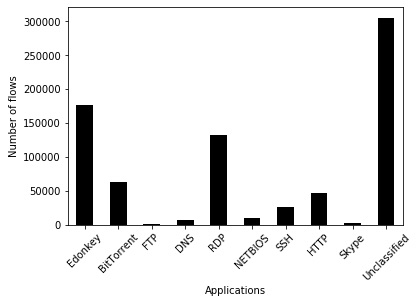
\includegraphics[width=3.6in]{fig1.jpg}
\caption{BroadBand Communication Research Group PCAP Data Flow}
\label{fig1}
}
\end{figure}

For the preprocessing of the supplied data, 8 kinds of application were selected based on the number of flows.
The 8 applications selected the application that has traffic of the actual network and the number of flow is more than 2000.
The 8 most common Label names are the Remote Desktop Protocol (RDP), Skype, SSH, Bittorrent, HTTP-Facebook, HTTP-Google, HTTP-Wikipedia and HTTP-Yahoo.
The application layer payload of the selected flow internal packet is filtered and extracted, and 8 application layer payload data files are generated using the extracted payload data.

\subsection{Learning Data Generation}\label
The process of converting the application layer payload data file created in the above section into input data suitable for deep learning learning will be described.
The application payload data file is divided into per packet unit and per flow unit, and each learning data is generated.
Flow is the same as the 5-tuple of the packet's header information, and packets generated within 3600 seconds of the previous packet are bundled into the same flow.
  
Each packet is extracted from each application layer payload data, and the elements of the payload data of the packet are grouped by 4 bits into one unit of learning data.
Therefore, one pixel of the learning data represents the number of 0 to 15.
One packet data collects pixelized data and image data as shown in Fig.\ref{fig2}.
One image data is converted into one packet learning data.

\begin{figure}[!t]
\centering
\setlength{\abovecaptionskip}{0pt}
\setlength{\belowcaptionskip}{0pt}
{
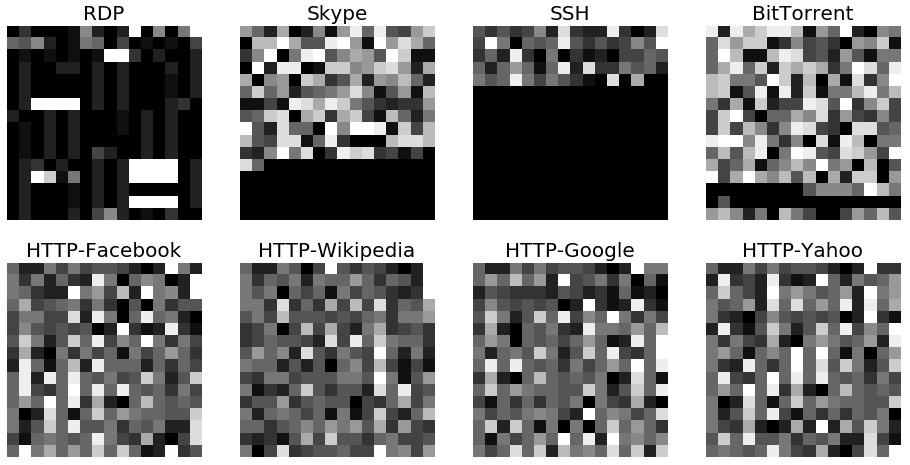
\includegraphics[width=3.6in]{fig2.jpg}
\caption{BroadBand Communication Research Group PCAP Data Flow}
\label{fig2}
}
\end{figure}

The learning data is generated by the packet unit and the flow unit for each application.
The learning data for each application per packet generates learning data by arbitrarily extracting packets of 8 applications (RDP, SSH, Skype, BitTorrent, Facebook, Wikipedia, Google, Yahoo) from the application layer payload data file.
In each application, 10000 random packets were extracted to extract a total of 80,000 learning data. One packet of each randomly extracted application is resized according to the size of the payload.
Therefore, the payload size of each application packet is extracted as 36 (6 * 6), 64 (8 * 8), 256 (16 * 16), and 1024 (32 * 32).
Figure 2 shows 16 * 16 of the payload data of an arbitrary packet for each extracted application.
If the extracted payload size is smaller than the set size, the size is adjusted by zero padding to match the set size.

The learning data of the flow unit is arbitrarily selected for each application in the application layer payload data file.
The selected flow fetches the packets from the first N packets as the number of packets (N) per predetermined flow.
They are  packets that has undergone a preprocessing process as in the learning data of each packet unit.
The learning data of the flow unit extracts 2000 flows for each application from the application layer payload data file and has a total of 16000 flows.
The number of N is set to 30, 60, and 100, and packets of each flow are fetched by the corresponding number to generate learning data.

Then, it is expressed as a one-hot vector with 8 lengths so that each of 8 applications can have label data.
A one-hot vector label is a vector with a value of only one element.
A one-value index can be defined as a label representing an application.
Therefore, two sets of learning data are used as the learning data packet or flow data and label data indicating the application data.

\section{Deep Learning Models}\label{sec:deeplearningmodels}
This chapter describes learning models that are used to classify network traffic using deep learning.
The Deep Learning model used is the Convolution Neural Network (CNN), the Residual Network (ResNet), the Recurrent Neural Network (RNN), the Long Short-Term Memory LSTM) and the Convolution and Recurrent Neural Network (CNN + RNN).
The Deep Learning model was supported by Keras, and the ResNet and CNN + RNN models were generated using Keras' CNN and RNN models simultaneously.

CNN and ResNet models are commonly used for information extraction, sentence classification, face recognition, and image classification.
CNN is a structure that extracts characteristics of data and grasps patterns of features.
In the case of RNN and LSTM, it is a model specialized for repetitive and sequential data learning.
Therefore, the previous learning data is reflected in the current learning using the circulation structure.
It is generally used for the composition of speech, wave and text.
Therefore, in the case of CNN and ResNet, it is used to classify using imaged packet unit data generated through preprocessing. RNN, LSTM, and CNN + RNN models are used to classify sequential data, so they are used to classify learning data in flow units that contain sequential information of network traffic.

\subsection{Convolution Neural Network Architecture}\label
A CNN model among the deep learning models for classifying network traffic will be described.
The model architecutre of CNN is composed of input layer, Convolution layer, and Pooling layer and Fully connected layer.
The input layer uses the payload and label of the packet converted into learning data. Packets are used as input data in the input layer in the form of $N \times N$ (N = 6, 8, 16, 32) like images.
Then, the feature of each packet data is convolved through the kernel of two Convolution layer, and output is generated through filter and activation process.
In the pooling layer, it is the process of reducing the size of the output through the convolution process.
It simply reduces the size of the data, cancels noise, and provides consistent features in fine detail.
Finally, the Fully connected layer extracts the prediction value according to the last 8 classes by activation.

Fig. \ref{fig3} is CNN architecture

\begin{figure}[t]
\centering
\setlength{\abovecaptionskip}{0pt}
\setlength{\belowcaptionskip}{0pt}
{
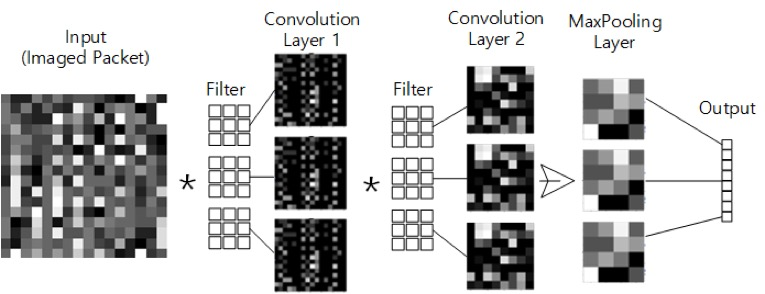
\includegraphics[width=3.6in]{fig3.jpg}
\caption{2-Layer Convolution Neural Network Learning Model}
\label{fig3}
}
\end{figure}

\subsection{Residual Network Architecture}\label
Unlike traditional CNN, ResNet [] has a unique concept called shortcut connection.
A shortcut connection is added to the existing CNN model structure, and this shortcut is directly connected without any other parameters.
A shortcut connection is a type of adding a new type of network to an input value so that learning can be performed.
Therefore, the newly added network can achieve better performance while maintaining the performance of the existing learned network as much as possible.

In terms of computation, there is nothing more than adding a compute operation.
Deep networks can be easily optimized through shortcut connections and can improve accuracy as depth increases.


\subsection{Recurrent Neural Network Architecture}\label
RNN is a network architecture that can accept inputs and outputs regardless of input data length, and can be implemented variously and flexibly as needed.
Therefore, the architecture of RNN used in this paper is composed of multi-layer as shown in figure 4.
In the RNN, the number of packets per flow (30, 60 and 100) is received at the input layer in order to learn flow unit data.
The number of units to be set is then output to the number of applications learned in the output layer through the RNN cell.

\subsection{Long Short-Term Memory Architecture}\label
In addition to the existing RNN model, LSTM determines whether to keep the weight value by adding another feature layer called a cell state.
Through this, we solve the phenomenon that the weight value is not maintained as the distance between information and information of one input data in the existing RNN becomes longer, and the learning ability decreases.
LSTM is more persistent than existing RNN because it keeps updating the past data.
The cell state is responsible for adding or deleting information.
The structure of the LSTM model is configured as shown in figure 5.
It is a single layer different from RNN.

The advantage of LSTM is that each memory control is possible and the result can be controlled.
However, there is a possibility that the memory may be overwritten, and the operation speed is slower than that of the conventional RNN.
Therefore, it is composed of single layer different from existing RNN model.

\subsection{CNN + RNN Architecture}\label
efefefef

\section{Model Tuning}\label{sec:modeltunning}
Each of CNN, RNN and LSTM models has various hyper-parameters which determines the network structure (e.g., number of filters) and how the network models are trained (e.g., type of optimizer).
The performance of the model can be greatly diverse according to the selected set of hyper-parameters.
In addition, the performance of the model may vary depending on the characteristics of the training datasets.
To do this, we use GridSearchCV, which is provided by Scikit-Learn, as a method of finding hyper-parameters optimized for each deep learning model according to the datasets.
The GridSearch method looks for the best hyper-parameter for a dataset by trying every possible combination of hyper-parameters based on the dataset.
GridsearchCV verifies the validity of the model by performing cross-validation in addition to finding the optimal hyper-parameters.
Cross-validation is a method of dividing specific data into training-only data and test-specific data, then using training data to learn, and testing with test data to verify the validity of the learning.
In this model tuning, we set the value of CV to 5 to find the optimal hyper-parameters and verify the validity of the model and hyper-parameters at the same time.

\subsection{CNN and ResNet Model Tuning}\label
The learning dataset of CNN and ResNet consists of packet unit data.
For each of the 8 applications, 10,000 packets were randomly organized into a single learning data set and the payload sizes of each packet were matched.
The payload size was divided by 36 (6 * 6), 64 (8 * 8), 256 (16 * 16), and 1024 (32 * 32) to increase the size of the dataset.
Therefore, the shape of the total training datasets is (80000, 6, 6, 1), (80000, 8, 8, 1), (80000, 16, 16, 1), (80000, 32, 32, 1).

There are a total of 15 hyper-parameters used in the CNN model provided by Keras.
Four of CNN hyper-parameters were selected.
{\it filter} represents the size of the output through one convolution layer, {\it kernel size} represents the size of the kernel used in the {\it filter}, {\it kernel initializer} represents the parameters for initializing the weight vectors of each layer, and {\it padding} represents the output of the Convolution layer.
It is necessary to fill in the pixel value specified by the outer angle of the input data with a specific value.
We perform GridSearch by adding {\it activation}, {\it optimizer}, and {\it batch size} which affects the whole learning in addition to the hyper-parameters to CNN.

Table 1 and 2 shows the values of the gridsearch performed for the selected hyper-parameter.
\begin{table}
\caption{The optimal CNN hyper-parameter values found by our grid-search}
\setlength{\tabcolsep}{3pt}
\begin{tabular}{|p{50pt}|p{35pt}|p{35pt}|p{47pt}|p{48pt}|}
\hline
 & $6 \times 6 (36)$ & $8 \times 8 (64)$ & $16 \times 16 (256)$ & $32 \times 32 (1024)$ \\
\hline
\hline
filter & 18 & 32 & 256 & 512 \\
\hline
kernel size & $3 \times 3$ & $5 \times 5$ & $5 \times 5$ & $3 \times 3$ \\
\hline
kernel initializer & glorot uniform & uniform & uniform & uniform  \\
\hline
padding & same & same & same & same  \\
\hline
activation & softmax & softmax & softmax & softmax \\
\hline
optimizer & adam & adam & adam & adam \\
\hline
batch size & 100 & 100 & 10 & 10 \\
\hline
\end{tabular}
\label{tab1}
\end{table}

\begin{table}
\caption{The optimal ResNet hyper-parameter values found by our grid-search}
\setlength{\tabcolsep}{3pt}
\begin{tabular}{|p{50pt}|p{35pt}|p{35pt}|p{47pt}|p{48pt}|}
\hline
 & $6 \times 6 (36)$ & $8 \times 8 (64)$ & $16 \times 16 (256)$ & $32 \times 32 (1024)$ \\
\hline
\hline
filter & 18 & 32 & 256 & 512 \\
\hline
kernel size & $3 \times 3$ & $7 \times 7$ & $5 \times 5$ & $7 \times 7$ \\
\hline
kernel initializer & glorot uniform & glorot uniform & uniform & glorot uniform  \\
\hline
padding & same & same & same & same  \\
\hline
activation & softmax & softmax & softmax & softmax \\
\hline
optimizer & adam & adam & adam & rmsprop \\
\hline
batch size & 100 & 100 & 100 & 100 \\
\hline
\end{tabular}
\label{tab2}
\end{table}

\subsection{RNN and LSTM Model Tuning}\label
The training datasets of SimpleRNN and LSTM is data of flow unit.
The training dataset was constructed by arbitrarily fetching 2000 flows from 8 applications.
In addition, the payload size of each flow unit packets has 36, 64, 256, and 1024, as packet unit.
The training data set of the flow unit is a data set that collects sequentially generated packets within the same 5-tuple and within 3600 hours.
The input data of the RNN must match the number of packets included in the flow.
Therefore, the number of packets per flow is set to 30, 60, and 100.
The final shape of the training data set is (16000, 30, 36), (16000, 30, 64), (16000, 30, 256) 16, 100, 256, 16000, 100, 36, 16000, 100, 64, 16000, 1024).

Keras The hyper-parameters used in RNN and LSTM models are 20 and the hyper-parameters of RNN and LSTM are the same.
We selected dual {\it units}, {\it kernel initializer}, {\it recurrent initializer}, and {\it dropout}.
{\it Units} represents the space of the output dimension, {\it kernel initializer} initializes the weight vector values of RNN and LSTM, {\it recurrent initializer} initializes the weight vector of recurrent state, {\it dropout} is a number between 0 and 1 It is a variable that deletes by the percentage of the number arbitrarily set in the number of units.
Like CNN, we perform GridSearch by adding {\it activation}, {\it optimizer}, and {\it batch size}.

Table 3 and 4 shows the values of variables that perform gridsearch for the selected hyper-parameter units, {\it kernel initailizer}, {\it recurrent initializer}, {\it dropout}, {\it activation}, {\it optimizer}, {\it batch size}.

%\begin{table}
%\caption{RNN hyper-parameter values}
%\setlength{\tabcolsep}{3pt}
%\begin{tabular}{|c|c|c|c|c|c|c|c|c|c|c|c|c|}
%\hline
% & \multicolumn{3}{$6 \times 6 (36)$} & \multicolumn{3}{$8 \times 8 (64)$} & \multicolumn{3}{$16 \times 16 (256)$} & \multicolumn{3}{$32 \times 32 (1024)$} \\
%\hline
% & 30 & 60 & 100 & 30 & 60 & 100 & 30 & 60 & 100 & 30 & 60 & 100 \\
%\hline
%\hline
%units & 128 & 128 & 64 & 256 & 128 & 64 & 256 & 128 & 128 & 128 & 128 & 64 \\
%\end{tabular}
%\label{tab3}
%\end{table}
%
%\begin{table}
%\caption{LSTM hyper-parameter values}
%\setlength{\tabcolsep}{3pt}
%\begin{tabular}{|p{50pt}|p{35pt}|p{35pt}|p{47pt}|p{48pt}|}
%\hline
% & $6 \times 6 (36)$ & $8 \times 8 (64)$ & $16 \times 16 (256)$ & $32 \times 32 (1024)$ \\
%\hline
%\hline
%filter & 18 & 32 & 256 & 512 \\
%\hline
%kernel size & $3 \times 3$ & $7 \times 7$ & $5 \times 5$ & $7 \times 7$ \\
%\hline
%kernel initializer & glorot uniform & glorot uniform & uniform & glorot uniform  \\
%\hline
%padding & same & same & same & same  \\
%\hline
%activation & softmax & softmax & softmax & softmax \\
%\hline
%optimizer & adam & adam & adam & rmsprop \\
%\hline
%batch size & 100 & 100 & 100 & 100 \\
%\hline
%\end{tabular}
%\label{tab4}
%\end{table}

\section{Experiments Evaluation}\label{sec:evaluation}
In this section, we compare packet-based application prediction and flow-unit application prediction.
CNN and ResNet are used for packet unit prediction.
RNN and LSTM are used for flow unit prediction.
In addition, we compare the performance of the model with the flow unit and the packet unit through the overall comparison of CNN, ResNet, RNN and LSTM.

\subsection{Experiments Environment}
The learning model is based on CNN, RNN, and LSTM supported by Keras 2.2.0.
In case of ResNet, network model was constructed using CNN model supported by Keras.
Model learning epochs were set to 200.

The experiments environment was run on Ubuntu 16.04 LTS, using 32GB of RAM and two NVIDIA GTX 1080Ti 11GB.
Experiments implementation uses version 1.8 of Tensorflow-gpu and version 2.2.0 of Keras in Python 3.6.
We were also able to utilize the GPU with CUDA 9.0 and CuDNN version 7.1.2.

The experiment performs Scikit-learn's GridSearchCV for one dataset and finds the optimal hyper-parameters through each model tuning.
The model learning was performed using optimal hyper-parameters for each dataset in Tables 1, 2, 3 and 4 of the Section.\ref{sec:modeltunning}.

\subsection{Performance Metrics}
In this paper, we use accuracy, precision, recall and f1-score for performance comparison of CNN, ResNet, RNN and LSTM models.
Accuracy, recall, precision, and f1-score provide performance metrics that take into account the unbalanced distribution of each application.
f1-score is the most important metric in all metrics.
f1-score represents the harmonic mean of precision and recall, and represents the classification performance of an unbalanced datasets.
The f1-score is expressed as 0 to 1 and is the best value at 1.

The definition of accuracy, precision, recall and f1-score follows four previous definitions as follow:
First, False Positive (FP) indicates that the prediction is that the application is correct, but not actually the application.
Second, False Negative (FN) indicates that the application is not expecting the result, but the application is actually correct.
Third, True Positive (TP) indicates that the application is correct and the application is correct.
Finally, True Negative (TN) indicates that the application is not the result of the prediction, but is not actually the application.
The definition of accuracy, precision, recall and f1-score according to the previous definition is as follows:

\begin{equation}
Accuracy =  \frac{TP + TN}{TP + TN + FP + FN}
\end{equation}

\begin{equation}
Recall =  \frac{TP}{TP + FP}
\end{equation}

\begin{equation}
Precision =  \frac{TP}{TP + FN}
\end{equation}

\begin{equation}
F1-score =  \frac{2 \times Precision \times Recall}{Precision + Recall}
\end{equation}

\subsection{Experiments Results}
The first experiment is a comparison of CNN and ResNet with the packet unit datasets.
In order to compare CNN and ResNet, the total f1-score was compared by varying the payload size of the packet to $6 \times 6 (36)$, $8 \times 8 (64)$, $16 \times 16 (256)$, and $32 \times 32 (1024)$.

\begin{figure}[t]
\centering
{
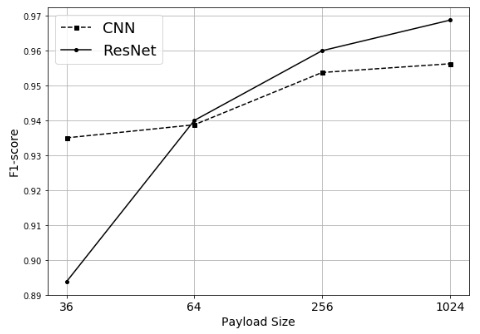
\includegraphics[width=3.4in]{fig7.jpg}
\caption{Comparison of CNN and ResNet with the overall f1-score for each application}
\label{fig7}
}
\end{figure}

Fig.\ref{fig7} compares f1-score for all applications by payload size in CNN and ResNet.
If the payload size of the packet is small, it can be seen that the overall f1-score value of CNN is about 0.4 higher than ResNet.
However, as the payload size increases, the training data set size also increases.
As a result, f1-score of ResNet is larger than CNN.
The reason is that because the learning model of ResNet is complex, less learning data sets are not good for learning.
Conversely, the larger the payload size and the larger the training data set, the better the performance of the more complicated ResNet model.

\begin{figure*}[h]
\centering
{
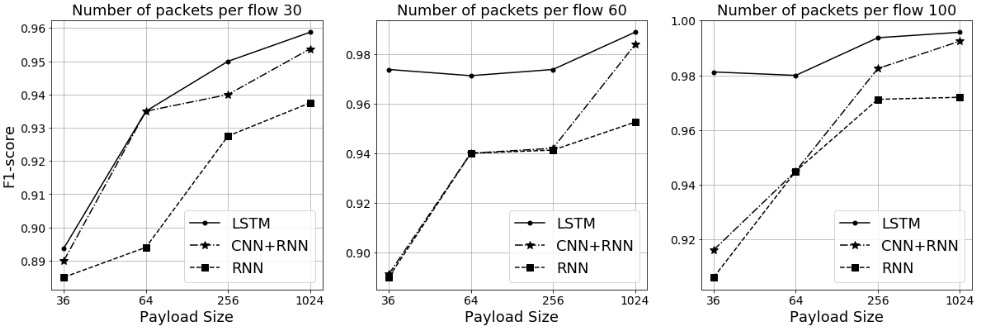
\includegraphics[scale=0.5]{fig9.jpg}
\caption{Comparison of RNN, LSTM and CNN+RNN with the overall f1-score for each application}
\label{fig9}
}
\end{figure*}

The following experiment is a comparison of RNN, LSTM, and CNN + RNN using flow unit datasets.
Fig.\ref{fig9} shows the total f1-score for each packet's payload size and the number of packets per flow.
It can be seen that the overall f1-score increases as the payload size of the packet increases.
Also, as the number of packets per flow increases, the entire f1-score increases.
When the number of packets per flow is 30 and the payload size is 36, the f1-score of each RNN, LSTM and CNN + RNN is 0.885, 0.89375 and 0.89.
However, when the number of packets per flow is 100 and the payload size is 1024, each f1-score thereof is 0.972, 0.99575 and 0.9925.
It is noticed that the f1-score across LSTM is higher than the total F1-score RNN and CNN + RNN.
It indicates that LSTM alone can provide similar or better performance without using complex models in the flow unit learning model.

\begin{figure}[t]
\centering
{
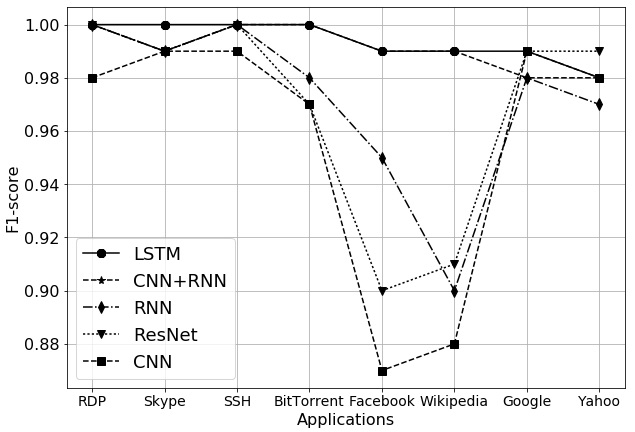
\includegraphics[width=3.3in]{fig10.jpg}
\caption{Comparison of packet unit classification and flow unit classification}
\label{fig10}
}
\end{figure}

Fig.\ref{fig10} is a graph comparing the f1-score results for each application when using a deep learning model to compare packet units and flow unit classifications.
In the case of CNN and ResNet, it represents the f1-score for each application when the payload size is $32 \times 32 (1024)$.
Also, in the case of RNN, LSTM, and CNN + RNN, it indicates the f1-score for each application when the payload size is 1024 and the number of packets per flow is 100.
Packet unit learning models CNN and ResNet show that f1-score on Facebook and Wikipedia are smaller than other applications.
The facebook and wikipedia packets are very similar to each other, so they are smaller than the f1-score of other applications' packets.
In the case of RNN, we can see that f1-score value of Facebook and Wikipedia are low as in the case of packet unit classification.
However, in the case of LSTM and CNN + RNN, the f1-score of both applications is high.
Thus, we can see that the LSTM and CNN + RNN learning models are well-categorized, and that the LSTM performs better with subtle differences.

\section{Conclusion}
\input{conclusion}





% if have a single appendix:
%\appendix[Proof of the Zonklar Equations]
% or
%\appendix  % for no appendix heading
% do not use \section anymore after \appendix, only \section*
% is possibly needed

% use appendices with more than one appendix
% then use \section to start each appendix
% you must declare a \section before using any
% \subsection or using \label (\appendices by itself
% starts a section numbered zero.)
%


\appendices
\section{Proof of the First Zonklar Equation}
Appendix one text goes here.

% you can choose not to have a title for an appendix
% if you want by leaving the argument blank
\section{}
Appendix two text goes here.


% use section* for acknowledgment
\section*{Acknowledgment}


The authors would like to thank...


% Can use something like this to put references on a page
% by themselves when using endfloat and the captionsoff option.
\ifCLASSOPTIONcaptionsoff
  \newpage
\fi



% trigger a \newpage just before the given reference
% number - used to balance the columns on the last page
% adjust value as needed - may need to be readjusted if
% the document is modified later
%\IEEEtriggeratref{8}
% The "triggered" command can be changed if desired:
%\IEEEtriggercmd{\enlargethispage{-5in}}

% references section

% can use a bibliography generated by BibTeX as a .bbl file
% BibTeX documentation can be easily obtained at:
% http://mirror.ctan.org/biblio/bibtex/contrib/doc/
% The IEEEtran BibTeX style support page is at:
% http://www.michaelshell.org/tex/ieeetran/bibtex/
%\bibliographystyle{IEEEtran}
% argument is your BibTeX string definitions and bibliography database(s)
%\bibliography{IEEEabrv,../bib/paper}
%
% <OR> manually copy in the resultant .bbl file
% set second argument of \begin to the number of references
% (used to reserve space for the reference number labels box)
\begin{thebibliography}{1}

\bibitem{IEEEhowto:kopka}
H.~Kopka and P.~W. Daly, \emph{A Guide to \LaTeX}, 3rd~ed.\hskip 1em plus
  0.5em minus 0.4em\relax Harlow, England: Addison-Wesley, 1999.

\end{thebibliography}

% biography section
% 
% If you have an EPS/PDF photo (graphicx package needed) extra braces are
% needed around the contents of the optional argument to biography to prevent
% the LaTeX parser from getting confused when it sees the complicated
% \includegraphics command within an optional argument. (You could create
% your own custom macro containing the \includegraphics command to make things
% simpler here.)
%\begin{IEEEbiography}[{\includegraphics[width=1in,height=1.25in,clip,keepaspectratio]{mshell}}]{Michael Shell}
% or if you just want to reserve a space for a photo:

\begin{IEEEbiography}{Michael Shell}
Biography text here.
\end{IEEEbiography}

% if you will not have a photo at all:
\begin{IEEEbiographynophoto}{John Doe}
Biography text here.
\end{IEEEbiographynophoto}

% insert where needed to balance the two columns on the last page with
% biographies
%\newpage

\begin{IEEEbiographynophoto}{Jane Doe}
Biography text here.
\end{IEEEbiographynophoto}

% You can push biographies down or up by placing
% a \vfill before or after them. The appropriate
% use of \vfill depends on what kind of text is
% on the last page and whether or not the columns
% are being equalized.

%\vfill

% Can be used to pull up biographies so that the bottom of the last one
% is flush with the other column.
%\enlargethispage{-5in}



% that's all folks
\end{document}


